% ============================================================
%  RESTRUCTURED 2026-08-16. This chapter is now the PROBLEM
%  STATEMENT: what is hard about this task and why it matters.
%  - "RAG Challenges and Solutions" moved IN from StateOfTheArt.tex
%    (the challenges you tackle are part of your problem, not the survey).
%  - The old "Solutions" bullet list was NOT moved: solutions belong to
%    the Proposition, where each is presented with its research + choice.
%  - Every "Approaches" subsection below is marked for MIGRATION into
%    the Proposition chapter; delete each one here once absorbed there.
% ============================================================

\chapter{The problem and its challenges} \label{ch:problem}

The core problem addressed in this research is the development of a Retrieval-Augmented Generation (RAG) implementation tailored for retrieving and synthesizing political text from Portuguese party manifestos. This involves overcoming challenges such as handling unstructured data, ensuring accurate retrieval, and generating contextually relevant responses. Below, we outline a proposed workflow for this implementation, as illustrated in Figure \ref{fig:my-rag-workflow}.

\TODO{Reword the problem statement so it reads as a research problem, not a
build task: the object of study is whether/how RAG techniques make long,
complex, low-resource-language civic documents genuinely accessible --- the
system is the instrument, not the goal. Also update "proposed workflow" +
figure: the pre-thesis naive-RAG diagram no longer matches the built system
(either update the figure or forward-reference
Figure~\ref{fig:system-overview}).}

\begin{figure}[h]
\begin{center}
    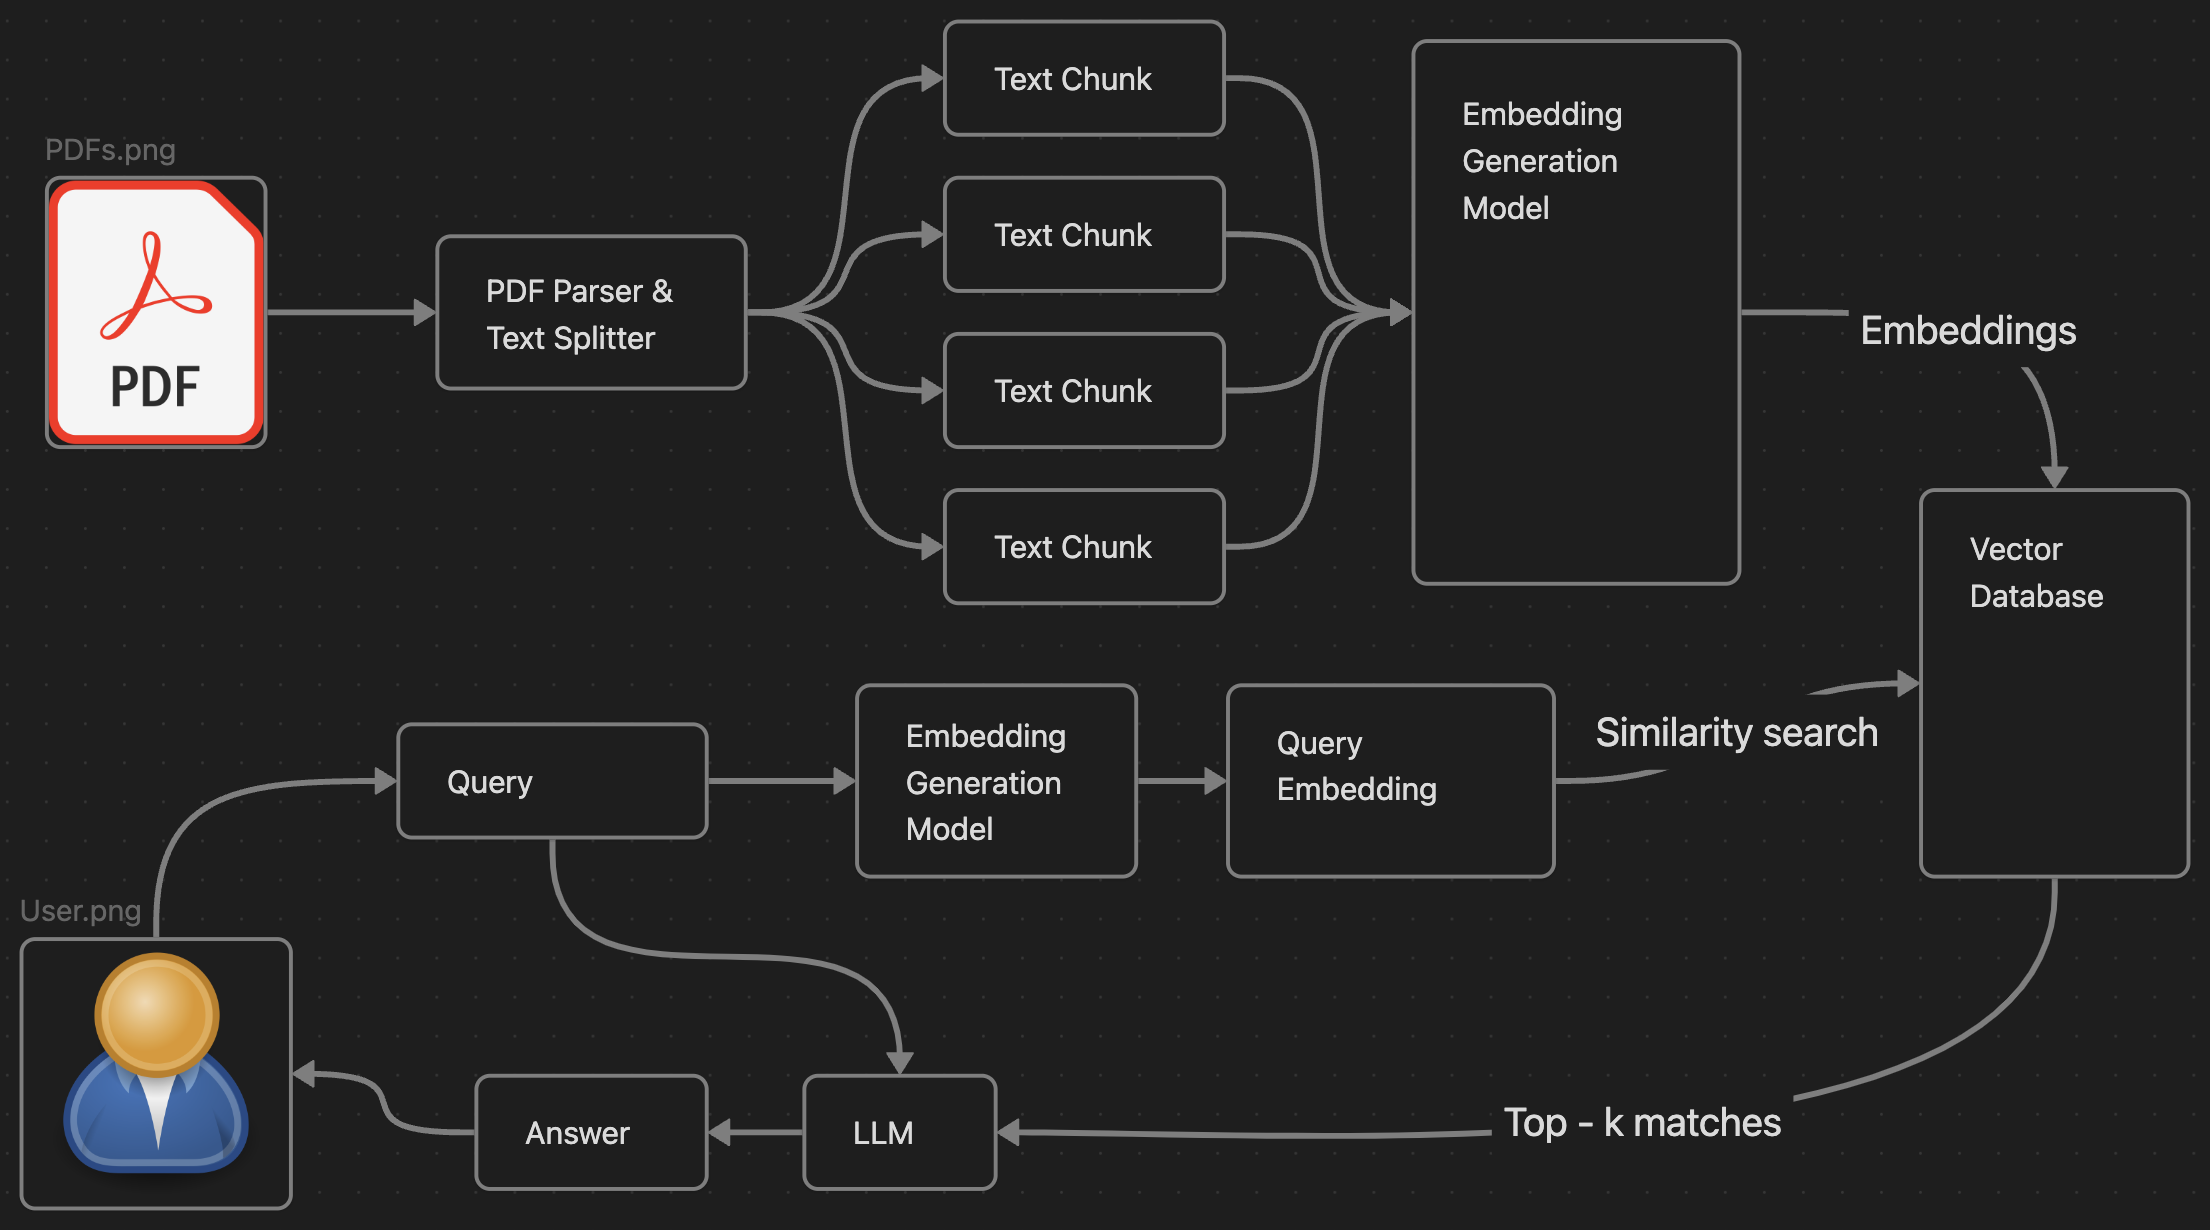
\includegraphics[width=0.8\textwidth]{images/my-RAG-workflow.png}
\end{center}
\caption{Simple RAG Workflow}
\label{fig:my-rag-workflow}
\end{figure}

\section{Challenges} \label{sec:challenges}
% Moved here from StateOfTheArt.tex — these are the problems this thesis tackles.

Despite its advancements, RAG faces several challenges when applied to real-world scenarios:

\begin{itemize}
\item \textbf{Messy Data:} Real-world data is often unstructured and heterogeneous, combining text, images, tables, charts, and diagrams. Extracting and processing such data, even from simple PDFs, can be challenging. Advanced parsing tools and multimodal approaches are needed to handle this complexity effectively.

\item \textbf{Inaccurate Retrieval:}
\begin{itemize}
    \item \textbf{Low Precision:} Retrieved documents often include irrelevant chunks, leading to hallucinations or the "lost in the middle" problem, where critical information is overlooked.
    \item \textbf{Low Recall:} Relevant chunks may be missed, leaving the model with insufficient context to generate accurate answers.
    \item \textbf{Outdated Information:} Retrieved data may be redundant or obsolete, reducing the reliability of generated responses.
\end{itemize}

\item \textbf{Bad Response Generation:}
\begin{itemize}
    \item \textbf{Hallucination:} Model makes up an answer that isn't in the context.
    \item \textbf{Irrelevance:} Model makes up an answer that doesn't answer the question.
    \item \textbf{Toxicity/Bias:} Model makes up an answer that's harmful, offensive or biased.
\end{itemize}

\item \textbf{Complex questions:} Some queries, though seemingly simple, require nuanced understanding and synthesis of multiple data points. For example, a question like "What is the current stance of left-wing parties on climate change?" may involve aggregating and interpreting data across multiple sources.
\end{itemize}

\TODO{Strengthen this list two ways. (a) Reword the generic challenges so each
one is anchored in YOUR corpus with a concrete example you actually hit ---
e.g.\ Messy Data $\rightarrow$ the manifesto layouts that broke parsing and
forced manual correction; Complex questions $\rightarrow$ a real multi-party
comparison query from your notes. (b) Consider adding domain-specific
challenges the generic list misses; candidates from your own project history:}
% Candidate additional challenges (suggestions to develop or discard):
%  - Low-resource language: European Portuguese specifically — most encoders
%    and benchmarks skew English or pt-BR; PT-specific models exist but are
%    trained for the wrong task (the serafim episode).
%  - Silent failures: components that degrade without erroring (encoder
%    truncation, ignored config flags) — hard to detect, directly harmed
%    retrieval quality; motivates the evaluation harness.
%  - Evaluation without ground truth: no PT manifesto QA dataset exists;
%    ground truth must be constructed, and it must survive re-indexing.
%  - Neutrality stakes: a civic-information tool must not distort party
%    positions; faithfulness matters more than fluency in this domain.
%  - Comparability across sources: 8 manifestos differ wildly in length,
%    structure and vocabulary; "compare X and Y" needs balanced retrieval
%    per party, not global top-k.
%  - Cost/scale constraints: academic budget, free-tier LLM rate limits —
%    they shaped real design decisions (checkpointing, optional
%    classification).

% ============================================================
% EVERYTHING BELOW: MIGRATE INTO chapters/Proposition.tex, THEN DELETE HERE.
% Each block names its destination. Do not leave duplicated text in both
% chapters in the final document.
% ============================================================

\section{Approaches} \label{sec:approaches}

\TODO{MIGRATION PENDING: this whole section dissolves into the Proposition ---
each subsection is the "candidates researched" half of the matching
Proposition subsection. Migrate block by block, then delete this section.}

% Data Collection, Embeddings and Vector Databases migrated to Proposition
% \ref{subsec:parsing}, \ref{subsec:embeddings}, \ref{subsec:vectorstore} (2026-10-06).

\subsection{Techniques to Improve RAG Retrieval}
% MIGRATE -> Proposition, split: metadata filtering -> \ref{subsec:routing};
% chunk size -> \ref{subsec:chunking}; reranking -> \ref{subsec:results} (scope
% decision) or future work; hybrid search -> \ref{subsec:search}; query
% translation/planning -> \ref{subsec:multiquery} and \ref{subsec:synthesis}

Several techniques can be employed to enhance the relevance and precision of retrieved documents, ensuring that the generator receives high-quality input. These techniques include metadata filtering, optimizing chunk size, reranking, hybrid search, and query translation, each addressing specific challenges in the retrieval process.

\subsubsection{Metadata Filtering or Routing}

Metadata filtering or routing is a technique that leverages additional information about documents — such as document type, creation date, source, or tags — to refine retrieval results. By incorporating metadata into the retrieval process, the system can prioritize documents that are more likely to be relevant to the query.

In the context of Portuguese political text analysis, metadata such as party affiliation, ideology, or policy domain can be used to filter or route documents. This ensures that the retrieved chunks are not only semantically relevant but also contextually appropriate. Metadata filtering can significantly improve retrieval precision, especially in scenarios where the dataset contains diverse or heterogeneous documents.

\subsubsection{Chunk Size}

The choice of chunk size plays a critical role in the performance of a RAG system, as it directly impacts retrieval accuracy and generation quality. Different chunk sizes present unique trade-offs, as illustrated in Table \ref{tab:chunk-sizes}.

\begin{table}[h]
    \centering
    \begin{tabular}{|c|c|}
        \hline
        \textbf{Small Chunk} & \textbf{Big Chunk}\\
        \hline
        More granularity & Less granularity \\
        More diverse sources & Less diverse sources \\
        Incomplete context & Lost in the middle problem \\
        \hline
    \end{tabular}
    \caption{Trade-offs in Chunk Size}
    \label{tab:chunk-sizes}
\end{table}

To address these challenges, the following steps are proposed:
\begin{itemize}
    \item \textbf{Evaluation Framework:} Define evaluation criteria to assess the impact of chunk size, including:
    \begin{itemize}
        \item Average Response Time (s)
        \item Average Faithfulness
        \item Average Relevancy
    \end{itemize}
    \item \textbf{Chunk Size Experimentation:} Test a range of chunk sizes (e.g., 128, 256, 512, 1024, 2048 tokens) to identify the optimal configuration for the specific use case.
\end{itemize}


\subsubsection{Reranking}

During a vector search, even when specifying a parameter like \texttt{top\_k=25} (to retrieve the 25 most relevant chunks), the returned chunks often vary in relevance and may not be sorted optimally. In practice, the most relevant chunks are frequently scattered across the retrieved set rather than being concentrated at the top.

Reranking addresses this issue by reordering the retrieved chunks based on their relevance to the query. This step ensures that the most pertinent information is prioritized, improving the quality of the input provided to the generator and, consequently, the accuracy of the final output. Techniques such as cross-encoders or learned ranking models can be employed to achieve this, leveraging additional context or metadata to refine the ranking process.

\subsubsection{Hybrid Search}

While vector search is powerful for capturing semantic relationships, it is not always the most effective method for every use case. In some scenarios, the desired information is better retrieved through keyword-based search, which excels at matching exact terms or phrases. Hybrid search addresses this limitation by combining the strengths of both vector and keyword search methods.

Hybrid search integrates the results from vector and keyword searches, merging them to produce a unified set of results. The top-ranked results from both methods are combined and reranked (see above), ensuring that the most relevant documents are prioritized. This approach is particularly useful for complex queries where both semantic meaning and specific keywords play a critical role.

\subsubsection{Query Translation/Planning}

Query translation or planning is a technique used to refine and optimize user queries for better retrieval performance. Complex or ambiguous queries can often lead to suboptimal results, as the retrieval system may struggle to interpret the intent behind the query. Query translation addresses this by breaking down complex queries into simpler sub-queries or rephrasing them to align more closely with the structure and content of the knowledge base.

For example, a query like "What are the economic policies of the major Portuguese political parties?" can be decomposed into sub-queries targeting specific parties or policy areas. Additionally, query planning can involve enriching the query with contextual information or synonyms to improve retrieval recall. This is something used by \cite{agentic-rag}.

By improving the alignment between queries and the knowledge base, query translation/planning enhances retrieval accuracy and ensures that the RAG system generates more relevant and precise responses.


\subsection{LLMs}
% MIGRATE -> Proposition: generation model choice belongs with
% \ref{subsec:synthesis} (or a short "model selection" note there); the
% judge-model discussion belongs in \ref{subsec:metrics}.

For this research, both open-source and proprietary LLMs are being considered, each offering unique strengths in terms of scalability, fine-tuning capabilities, and performance on low-resource languages like Portuguese. The following models are under evaluation:

\begin{itemize}
    \item \textbf{Open-Source Models:}
    \begin{itemize}
        \item \texttt{Llama 3.3 70B:} A state-of-the-art open-source model developed by Meta.
        \item \texttt{DeepSeek-V3:} A recent and versatile open-source model optimized for multilingual tasks, including low-resource languages like Portuguese.
    \end{itemize}
    \item \textbf{Proprietary Models:}
    \begin{itemize}
        \item \texttt{OpenAI's GPT-4:} A highly advanced proprietary model renowned for its ability to generate human-like text and handle complex queries with high accuracy.
        \item \texttt{Google's Gemini 2.0 Flash:} A cutting-edge model designed for fast and efficient text generation, particularly suited for real-time applications.
    \end{itemize}
\end{itemize}
